\usetikzlibrary{patterns}
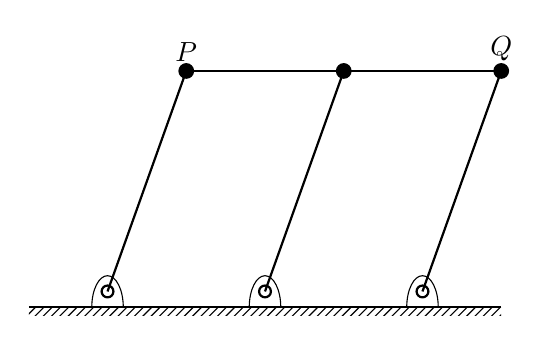
\begin{tikzpicture}
    \coordinate (P) at (0,2);
    \coordinate (Q) at (4,2);
    \coordinate (A) at (-1,-0.8);
    \coordinate (B) at (3,-0.8);
    \coordinate (C) at (1,-0.8);
    \coordinate (M) at (2,2);

    \draw[thick] (-2,-1) -- (4,-1);
    \fill[pattern=north east lines] (-2,-1) rectangle (4,-1.1);

    \draw[thick] (P) -- (A);
    \draw[thick] (Q) -- (B);
    \draw[thick] (P) -- (M) -- (Q);
    \draw[thick] (M) -- (C);

    \draw[thick] (-1,-0.8) circle(0.075);
    \draw[thick] (3,-0.8) circle(0.075);
    \draw[thick] (1,-0.8) circle(0.075);

    \draw[draw=black] (-0.8,-1) arc[start angle=0, end angle=180, x radius=0.2cm, y radius=0.4cm];
    \draw[draw=black] (3.2,-1) arc[start angle=0, end angle=180, x radius=0.2cm, y radius=0.4cm];
    \draw[draw=black] (1.2,-1) arc[start angle=0, end angle=180, x radius=0.2cm, y radius=0.4cm];

    \fill (P) circle(0.1);
    \fill (Q) circle(0.1);
    \fill (M) circle(0.1);

    \node[above] at (P) {$P$};
    \node[above] at (Q) {$Q$};
\end{tikzpicture}
